% Porfavor no cambiar el formato, este es el exigido por el Encuentro Chileno de la Computacion.
% Mantenerlo así hasta el 15/07/2008.
% Idioma: español, inglés o portugués.
% Tamaño 8 1/2" x 11" (carta, letter USA), máximo 10 páginas, incluyendo resumen no superior a
% 130 palabras.
% Márgenes: superior 3,5 cm, inferior 2 cm, derecho e izquierdo: 2,5 cm.
% Formato: Texto justificado a la derecha e izquierda, páginas no numeradas.
% Tipo de letra: Times 10 para el texto y 12 para títulos y apartados.
% La primera página debe contener: El título del trabajo, nombre completo de autores, afiliación y
% direcciones, así como el resumen del trabajo y palabras claves para su clasificación sobre la base de
% los temas propuestos en este llamado.

\documentclass[conference]{IEEEtran}
\usepackage{graphicx}
\usepackage{url}
\usepackage[utf8]{inputenc}
\usepackage{enumerate}

%opening
\title{Titulo}

\author{
\IEEEauthorblockN{
Rodrigo G. Fernández\IEEEauthorrefmark{1}
}
\IEEEauthorblockA{
\IEEEauthorrefmark{1}Computer Systems Research Group~\cite{CSRG}, Universidad Técnica Federico Santa María, Av. ~España~1680, Valparaíso, Chile
%\IEEEauthorrefmark{2}Centro de Robótica~\cite{CR}, Universidad Técnica Federico Santa María, Av. ~España~1680, Valparaíso, Chile
}
}
\begin{document}
\bibliographystyle{plain}
\pagestyle{empty}

\maketitle\thispagestyle{empty}

\begin{abstract}
Este documento presenta
%el avance y proceso de creación de una aplicación que permita desarrollar las
%rutinas de control para diferentes tipos de plataformas robóticas, unificando los diferentes mecanismos de comunicación
%con cada dispositivo en un solo lenguaje de programación, buscando simplificar la programación de las
%plataformas robóticas y hacer más eficiente el trabajo del investigador.
%Dentro de las consideraciones se encuentran: (a) la elección de un lenguaje estandarizado que posibilite un fácil
%aprendizaje y permita realizar una amplia gama de tareas; (b) la estructura del software a desarrollar, y (c)
%la perduración del mismo en el tiempo.
%Tras haber considerado todos estos puntos, se estableció que nuestro software sería desarrollado en
%Python, con una estructura modular y extensible utilizando archivos XML, y de código abierto.
%Se presentan resultados parciales sobre el desarrollo del proyecto y del software.
\end{abstract}

\textbf{Palabras Clave:} Testing, Desarrollo de Software

\section{Introducción}
\label{sec:intro}
% Esta mala, falta revisarla una vez terminar el paper.

El siguiente documento tiene como objetivo principal, 
%presentar el estudio realizado en distintas plataformas robóticas,
%particularmente Arduinos~\cite{ARDUINO},
%teniendo como finalidad sustentar en forma sólida,
%el desarrollo de la solución a la siguiente problemática: \\

\emph{
Actualmente,
 (...) ,
se tiene como finalidad:
\begin{enumerate}[a.]
    \item 
\end{enumerate}
}

Por tal motivo, en el presente documento se detallarán los siguientes puntos:

\begin{itemize}
	\item Señalar la problemática que actualmente afecta al 
    %Centro de Robótica UTFSM, centro de investigación con el cual se está trabajando en forma colaborativa, para poder establecer un Software que supla las necesidades reales.
	\item Detalle de todas las posibles alternativas que darían solución a 
    %la problemática planteada anteriormente, las cuales fueron analizadas con el fin de desarrollar la más óptima.
	\item Descripción de distintos tipos de técnicas de
    %desarrollo de software, utilizado para construir la solución.
	\item Método de implementación de 
    %la solución a desarrollar.
\end{itemize}

El presente trabajo se divide como sigue:
En la sección~\ref{sec:definicion}
%acota la problemática de la programación de plataformas robóticas, 
%haciendo notar las dificultades que se tienen al llevar a cabo esta tarea.
La sección~\ref{sec:estado} muestra un resumen de los trabajos
%que se han realizado en torno a este problema,
%y las distintas aproximaciones que se han adoptado en el último tiempo.
En la sección~\ref{sec:objetivos}
%se muestran los delineamientos del trabajo que se realizará
%dentro de este proyecto.
La sección~\ref{sec:metodo} muestra cómo se lleva a cabo el proyecto,
%cuales han sido las principales decisiones,
%y cómo se avanzará.
En la sección~\ref{sec:resultados}
%se muestran los resultados obtenidos hasta el momento
%en cuanto al desarrollo de la interfaz
%y los puntos trabajados en conjunto con el Centro de Robótica UTFSM.
La sección \ref{sec:conclusiones} presenta un resumen
%y consideraciones de nuestro trabajo a la fecha,
%además de enfocarse a delinear el futuro de nuestro proyecto.


\section{Contextualización del Problema}
\label{sec:definicion}
Hoy en día,
%cada vez se realizan más y mejores investigaciones en el área de la robótica,
%tanto a nivel nacional como internacional.

La evolución de 
%las plataformas robóticas industriales desde sus principios ha sido vertiginosa.
%En poco mas de 30 años las investigaciones y desarrollos sobre robótica industrial,
%han permitido que los robots tomen posiciones en casi todas las áreas productivas y tipos de industria.

La manipulación de 
%dispositivos complejos ha dejado de ser una problemática sólo para las grandes
%empresas del rubro.
%El avance en las técnicas de la robótica y la difusión de la tecnología han dado como resultado,
%que la construcción de un dispositivo robótico,
%también sea un desafío para estudiantes e investigadores.

Las pocas soluciones existentes a la hora de implementar 
%interfaces de control,
%para este tipo de aparatos son de dos tipos:
%Aquellas que son propiedad de las empresas que fabrican las piezas de los dispositivos,
%y las que son implementadas por el propio equipo de desarrollo.
%En el primer caso,
%estas interfaces suelen ser muy restrictivas y poco flexibles;
%en el segundo caso,
%son muy rústicas y requieren la dedicación de recursos humanos y tiempo valioso para el equipo,
%que no se encuentra entre las metas del dispositivo en desarrollo.
%Todo esto limita el desarrollo de mejores aplicaciones y la experimentación con diferentes modelos.

Por otro lado, debido a todas las problemáticas actuales,
es fundamental 
%desarrollar una interfaz de control que las solucione,
%unificando las diferentes herramientas y optimice los recursos para la investigación de nuevas tecnologías.

A continuación, en la Figura 1, se señalan las fases por las cuales,
%cualquier investigador debe pasar,
%para poder probar una rutina determinada en una plataforma robótica:
%
%\begin{figure}[htp]
%	\begin{center}
%		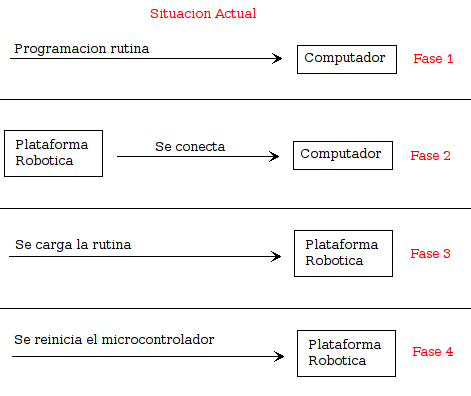
\includegraphics[scale=0.7]{img/user-sist}
%		\caption{Comunicación y perturbaciones}
%	\end{center}
%\end{figure}

\subsubsection{Identificación de problemas y deficiencias}
Debido a la situación anteriormente planteada,
se identificaron las siguientes problemáticas: 
\begin{itemize}
    \item 
\end{itemize}

\subsection{Caracterización del cambio}

\subsubsection{Características y potencialidades deseadas}
	Se espera que el sistema a desarrollar posea y/o sea capaz de:
%	\begin{itemize}
%		\item \textbf{Interfaz Gráfica de Usuario:}
%				
%		\item \textbf{:}
%
%		\item \textbf{Alta Modularidad:}
%			Con respecto a la construcción en sí del \emph{software},
%			se desea que ésta sea de carácter modular, para poder distribuir de manera más óptima,
%			las distintas funcionalidades que son necesarias para las plataformas robóticas que posee nuestro nicho 
%			de investigación, el Centro de Robótica de la UTFSM,
%			facilitando la implementación de funcionalidades futuras y compatibilidad con nuevos modelos del rubro.
%
%		\item \textbf{Portable a otros sistemas Operativos:}
%			Es necesario, no restringir una aplicación que busca suplir un problema tan importante en el área de la
%			robótica a un solo tipo de Sistema Operativo, por lo que se requiere utilizar herramientas que posibiliten
%			en el futuro poder portar la aplicación a diferentes plataformas computaciones (por ejemplo, Linux OS, Windows OS, etc)
%
%		\item \textbf{Estándar para el desarrollo de nuevos controladores, funcionalidades y aplicaciones:}
%			Además,
%			para que el sistema pueda seguir creciendo a diferentes y nuevos dispositivos,
%			es necesario que existan estándares para el desarrollo de nuevos componentes del sistema.
%
%		\item \textbf{Código Abierto:}
%			Para mantener la idea de que el sistema se pueda ampliar y desarrollar más allá de lo que dure nuestro proyecto,
%			es necesario que el mismo se rija bajo licencias que mantengan el código abierto a toda la comunidad.
%			Por ello,
%			éste se licenciará bajo la \emph{General Public Licence (GPL)}~\cite{GPL},
%			que resguarda y valida al proyecto en frente a la comunidad internacional.
%	\end{itemize}

La importancia de poder solucionar este tipo de problemas,
es que 
%el desarrollo en el área de la robótica en nuestro país,
%si bien es cierto, ha tenido variados avances, no está al nivel de países desarrollados
%que presentan las últimas vanguardias en el área.
%El desarrollo de Software es un tema clave a nivel de investigación en distintas áreas,
%pues potencia la calidad y ayuda a poder realizar investigaciones y desarrollos de una forma
%más expedita.

%Automatizando distintos procesos en el área de la investigación de la robótica,
%se está logrando que los especialistas que se desarrollan en éste ámbito,
%puedan no perder el tiempo con procedimientos que no tengan un gran significado,
%enfocándose sólo en aspectos mas importantes,
%dejando un poco de lado procesos de almacenamiento, tratamiento e interpretación de información.

% Conclusion
Por el hecho de que 
%en Chile existen distintos escenarios,
%donde prima la investigación en el área de la robótica,
%se está enfrentando una problemática latente.

El problema es complejo,
%tanto que existen varias empresas que encuentran rentable
%el desarrollo de software en esta área.


\section{Estado del Arte}
\label{sec:estado}
El trabajo de los investigadores del área de 
%la robótica fuera del diseño del robot en sí,
%es lidiar con el problema de encontrar y/o desarrollar un medio a través del cual interactuar con él.
%Una de las posibles soluciones a las que pueden recurrir, es la reutilización de software,
%sin embargo, esta no es una tarea sencilla~\cite{wcam-1}, ya que es necesario entender el código
%y además adaptarlo a nuestro sistema, tarea que requiere tiempo, el cual podría ser mejor aprovechado
%en otros aspectos de la misma investigación.

Otra de las soluciones actuales es 
%buscar un software que unifique la
%comunicación y la interacción con el robot~\cite{wcam-4}.

Actualmente existen distintas soluciones de software para el estudio de 
%robots, soluciones que van desde
%reproducir sus movimientos a través de la realización de simulaciones de las diferentes plataformas, hasta 
%la implementación de interfaces para la programación y comunicación.

Un punto importante a la hora de realizar comparaciones entre diferentes
aplicaciones es 
%que los enfoques de solución que utilizan son distintos y como
%es señalado en~\cite{wcam-4} se termina intentando realizar una comparación
%entre cosas esencialmente muy diferentes.

Por otro lado, en algunas soluciones,
%como Pyro~\cite{PYRO}, se puede apreciar
%una escasa aplicación de ingeniería de software, debido a la poca preocupación
%por la interfaz de manejo sin aprovechar las facilidades que las tecnologías
%actuales ofrecen, dificultando el trabajo de fondo innecesariamente.

Hay un punto a destacar en el ámbito de 
%los simuladores, en el cual si bien se trata de generar un
%ambiente en el que se desenvuelve una plataforma robótica, de la manera más real posible, nunca se podrá
%determinar todas las posibles variables que pudiesen afectar algún tipo de experimento, por lo que
%idealmente se puede generar un entorno reduciendo variables, logrando así limitar el problema, pero
%dejando de lado toda realidad.

Referente a la propiedad intelectual del software relacionado a la investigación del área de 
%la robótica,
%se está enfrentando a dos grandes tendencias, por un lado se tiene al software OpenSource~\cite{OPENSOURCE}, 
%el cual hace referencia al software que posee características de ser distribuido,
%desarrollado, obtenido e incluido libremente, entre otras características; por el otro lado se encuentra
%el software propietario, el cual limita las posibilidades de usarlo, modificarlo o
%redistribuirlo con o sin modificaciones, como lo es Microsoft Robotics Developer Studio~\cite{MICROSOFT}.
%Dada las características de cada tendencia, se ve que OpenSource permite establecer, dada sus
%características, un total apoyo a la libre investigación y aporte a los diferentes softwares.


\section{Objetivos}
\label{sec:objetivos}
Los siguientes son los objetivos que han sido planteados a completar hasta
%diciembre del presente año:

\subsection*{Objetivo General}

\subsection*{Objetivos Específicos}
\begin{itemize}
    \item
\end{itemize}


\section{Metodología}
\label{sec:metodo}
Hoy en día existen muchas aplicaciones y recursos robustos para poder solucionar
distintos problemas enfocados al estudio y análisis de 
%plataformas robóticas.

Para desarrollar este proyecto fue necesario detectar cuáles de estos recursos
son los que permitirían
%crear una Interfaz Gráfica de Usuario (GUI) que pueda ofrecerle
%a los investigadores una alternativa que facilite su labor.

Por tanto, fue una necesidad el realizar un estudio de 
%las herramientas que otras interfaces
%ofrecían \footnote{\emph{Descritas posteriormente en VI. Resultados, subsección A}}, cumpliendo así una
%labor similar, tomando en cuenta que nuestro proyecto define como
%usuario final a desarrolladores e investigadores interiorizados en el área de la robótica.

Para poder obtener dicha información fue necesario 
%dirigirnos al origen de la problemática y establecer
%un trabajo en conjunto con las personas dedicadas al área de la robótica. En nuestro caso, la
%investigación se ha realizado en conjunto con el Centro de Robótica de la UTFSM. Ésto 
%ayudó a definir correctamente el enfoque que se tendría que dar al proyecto, tanto por el lado de
%los requerimientos principales de nuestro proyecto, como de la interfaz que un investigador de esta área
%espera encontrar para, finalmente, facilitar la realización de la investigación en las plataformas
%robóticas.

%PROPÓSITO: CONVENCER A UNA AUDIENCIA TÉCNICA QUE SE SABE CÓMO CONSTRUIR LA SOLUCIÓN.
Es en base a este enfoque que, después de realizar una investigación sobre las diferentes herramientas,
se decidió
%para el proyecto utilizar el lenguaje de programación Python, por el entorno de trabajo
%que nos ofrece, permitiéndonos generar soluciones rápidamente y ser un lenguaje multiparadigma fácilmente
%extensible.
%Además, posee bastantes facilidades para trabajar en la implementación de interfaces de éste tipo, ya que
%contiene una gran cantidad de bibliotecas para el manejo de diferentes aspectos del proyecto, como la
%comunicación serial (pySerial~\cite{PYSERIAL}),
%creación de algoritmos, y comunicación con la interfaz gráfica (pyQt~\cite{PYQT}), la cual junto a bibliotecas
%específicas, ofrece herramientas con un entorno para desarrollar Interfaces
%Gráficas de Usuario (Qt Designer~\cite{QTDESIGNER}).

Para 
%las bibliotecas gráficas, se optó por utilizar QT, al ser de fácil implementación en conjunto con Python (pyQt) y por su gran portabilidad
%entre diferentes sistemas operativos.
Finalmente,
%para todo lo que significa la configuración de las plataformas
%robóticas, se utilizó XML, por ser un estándar para el intercambio de
%información estructurada entre diferentes plataformas, además de poseer la ventaja
%de ser extensible para poder modificar y usar sus datos sin mayores
%complicaciones. De esta manera, se reduce la dificultad de aprendizaje y
%facilita el trabajo para que personas externas puedan aportar al
%desarrollo del proyecto.

Para desarrollar el presente trabajo, se han escogido métodos 
%ágiles, sobre todo en extreme programming~\cite{XP},
%por los principios que la sustentan; \emph{simplicidad, comunicación, retroalimentación y coraje}\cite{xp-book}.

Para complementar y corregir las deficiencias del presente proyecto,
%se utiliza como sistema de seguimiento de desarrollo de software a
%Trac~\cite{TRAC}, el cual integra una wiki, un repositorio GIT~\cite{GIT} y
%herramientas para el seguimiento y control de tareas. Esto permitió un rápido
%avance en las tareas del grupo, pues cada integrante podía estar al tanto de
%las actividades de sus compañeros de equipo, sin necesidad de mantener
%reuniones presenciales. Cabe mencionar que ésta metodología de trabajo
%nos fue de fácil implementación, gracias a que cada uno de los miembros del
%equipo se encontraban previamente familiarizados con las herramientas utilizadas, a que
%las tareas a realizar eran fácilmente identificables y que comenzadas las
%etapas de desarrollo no requerían de un gran trabajo en conjunto.


\section{Resultados}
\label{sec:resultados}
El primer resultado
%Del proyecto fue la revisión de funcionalidades indispensables que debe poseer una
%Herramienta para el control de dispositivos complejos como los robots con variados grados de libertad, lo
%Cual llevó al equipo de trabajo a hacer un estudio y diseño de la interfaz de manejo que facilite la interacción máquina –
%Hombre.

%\subsection{Análisis de las herramientas existentes}
%\begin{itemize}
%	\item Player~\cite{PLAYER}\\
%		Es un servidor de red para control de robots. Este se ejecuta en el robot, y provee una interfaz hacia
%		los sensores y otros dispositivos a través de una red IP. El programa cliente se comunica con Player a
%		través de un socket TCP, leyendo la información de los sensores, escribiendo y configurando dispositivos
%		en el proceso. Es el estándar de facto en la comunidad robótica de código abierto, y se ha desarrollado
%		como un poderoso robot framework~\cite{wcam-5}.
%		Soporta una gran variedad de hardware de robots, y al ser su arquitectura modular, hace fácil el agregar soporte
%		a nuevos dispositivos, y posee una comunidad activa que contribuye con nuevos controladores.
%		Entre las características que posee:
%		\begin{itemize}
%			\item Soporta virtualmente variados clientes a la vez.
%			\item Los clientes puede conectarse y leer los datos de los sensores de variadas instancias de Player en cualquier robot.
%			\item Posee dos herramientas, Stage~\cite{STAGE} y Gazebo~\cite{GAZEBO}, para realizar pruebas con robots virtuales en 2 dimensiones y 3 dimensiones, respectivamente.
%			\item Es software libre licenciado bajo la GNU Public License.
%		\end{itemize}
%		
%		Es bastante versátil y ofrece bastantes posibilidades para desarrollar el robot, pero está centrado al
%		control y comunicación más que al entorno de desarrollo del investigador. A pesar de estar basado en el
%		protocolo TCP para dar mayores libertades de trabajo y más simplicidad a la hora de programar, posee una
%		instalación bastante compleja y poco portable.
%
%	\item Carmen~\cite{CARMEN}\\
%		 	Carmen es una colección de software OpenSource para el control de robots móviles. Es un software modular
%		diseñado para proveer navegación básica en elementos primitivos incluyendo: control de bases y sensores, logging, 
%		evasión de obstáculos, localización, planes de rutas, y mapeo. La comunicación entre los procesos Carmen es manejada
%		utilizando IPC (Inter process communication).
%		Entre las características que posee:
%		\begin{itemize}
%			\item Software de control de robots modular.
%			\item Utilización de plataforma IPC para comunicación entre procesos.
%			\item Soporte de hardware robótico para diferentes plataformas.
%			\item Monitor de procesos.
%			\item Servidor centralizado de parámetros.
%			\item Hecho en C, pero provee soporte para Java.
%			\item Módulo de localización. 
%			\item Simulador de robots y sensores.
%			\item Módulo de planeación de ruta.
%		\end{itemize}
%		Lo que convierte a Carmen en una herramienta bastante completa, 
%		en lo que se refiere a plataformas móviles.\\
%
%	\item YARP~\cite{yarp-paper}\\
%		Es un conjunto de bibliotecas, protocolos y herramientas con la finalidad de mantener
%módulos y dispositivos desacoplados, de la manera más limpia posible. Una situación que comúnmente se da
%en el área de la robótica, es que la evolución de los proyectos termina debido a dependencias de
%bibliotecas obsoletas, dispositivos de hardware poco comunes y reducción del personal humano a cargo, de
%por sí ya mínimo. Yarp tiene la intención de establecer un software duradero y estable~\cite{wcam-2}, evitando generar
%restricciones relacionadas con cambios de hardware específico, con la consecuente ventaja de concentrar
%los esfuerzos en la organización de los dispositivos. Yarp es OpenSource~\cite{OPENSOURCE}, por lo
%que posee la cualidad de ser escrito por investigadores para investigadores.\\
%
%Principales componentes de Yarp:
%
%\begin{itemize}
%
%\item libYARP\_OS: Interfaz para ser utilizado con el Sistema Operativo, permitiendo dar el correspondiente soporte para la comunicación de datos entre diferentes tareas en muchas máquinas, independiente del Sistema Operativo en el que se encuentre alojado.
%\item libYARP\_sig: Realiza tareas comunes en el ámbito del procesamiento de señales, tanto audio
%visuales como auditivas, con facilidad de uso con otras bibliotecas, como OpenCV~\cite{OPENCV}.
%\item libYARP\_dev: Provee una interfaz común con dispositivos como cámaras, tableros de control, motores, etc.
%\end{itemize}
%
%
%\end{itemize}
%
%
%\subsection{Primeras Versiones de $\mu$Bot Interface~\cite{ubot}}
%
%Hasta el momento, se ha logrado desarrollar una Interfaz Gráfica de Usuario (GUI) capaz de proveer
%varias funcionalidades del sistema de control, dentro de las cuales se encuentran:
%\begin{itemize}
%	\item Wizard de configuración para configurar la plataforma robótica a utilizar.\\
%		Provee la facilidad necesaria al momento de dar el primer paso, en el
%		contexto de definir la plataforma robótica a utilizar. Permite establecer
%		desde cosas sencillas como el identificador único que posee la configuración
%		de dicha plataforma, hasta la selección del tipo de microcontrolador que
%		posee, dando además la factibilidad de seleccionar los distintos dispositivos
%		que posee la plataforma e indicar en que pin se encuentra conectado cada uno.
%
%	\item Visualización de los dispositivos configurados.\\
%		Permite observar en una manera totalmente rápida y expedita, toda la
%		información referente a los dispositivos configurados (previamente conectados
%		a la plataforma robótica), desde el tipo o familia a la que pertenece cada
%		dispositivo, en que pin se puede establecer conexión hacia él, hasta
%		características propias de dicho dispositivo, como rangos de funcionalidad de
%		motores. 
%
%	\item Consola Python.\\
%		Debido a que toda la información interna de la plataforma robótica es
%		accesible mediante la utilización de orientación a objetos, gracias a la
%		implementación propia de nuestra interfaz, se cuenta con una consola Python,
%		que permite aprovechar las ventajas anteriormente mencionadas, además de
%		contar con toda la riqueza del lenguaje Python, permitiendo así brindarle al
%		programador una capa de abstracción mucho más acorde a la de un investigador,
%		evitando la comunicación a bajo nivel con las plataformas.
%
%	\item Editor Python.\\
%		Debido a que se cuenta con la consola Python, es posible desarrollar
%		todo el código que se estime conveniente en lenguaje Python, por lo que el
%		editor provee una manera rápida y expedita para realizar ésto, teniendo al
%		alcance ambas herramientas interactuando entre sí. 
%
%	\item Envío de instrucciones a la plataforma robótica por puerto serial/usb.\\
%		El envío de instrucciones se facilita gracias a la orientación a
%		objetos que se implementó, de este modo es posible acceder a las
%		funcionalidades de cada dispositivo y a su vez, obtener la información de
%		salida que éstos provean.
%
%	\item Rutinas predeterminadas.\\
%		Para reducir la complejidad de los diversos movimientos que puede tener un
%		robot, se piensa integrar a la interfaz la capacidad de generar rutinas de
%		movimiento básicas para algunas plataformas robóticas para así disminuir
%		tiempo utilizado en el desarrollo de aplicaciones o estudios relacionados con
%		la robótica, sin dejar de lado la transparencia y simplicidad de la
%		comunicación con el robot. 
%
%	\item Integración con proyecto GEAR.\\
%		Todo lo anteriormente señalado, no sería posible si no se contara con el
%		proyecto \cite{GEAR}, que provee en un nivel de abstracción mucho más alto,
%		para poder realizar una interacción con distintas microcontroladores,
%		y así poder contar con un ciclo completo, al momento de desarrollar
%		rutinas de control entre nuestro proyecto y distintas plataformas robóticas.
%		Actualmente, el proyecto GEAR permite la comunicación con tres
%		microcontroladores; Arduino (ATmega328), Sanguino (ATmega644) y ArduinoMega), 
%		los cuales son los que se han utilizado para las pruebas del software.
%\end{itemize}
%


\section{Conclusiones}
\label{sec:conclusiones}
\begin{frame}
\frametitle{Conclusiones}
\begin{itemize}
    \item 
\end{itemize}
\end{frame}



%\section*{Agradecimientos}
%
%  Este trabajo es financiado por
% (...)
%  Por otro lado, los autores agradecen el apoyo de CSRG  (Computer Systems Research Group)
%del Departamento de Informática de la UTFSM, por facilitarnos su infraestructura y respaldo en el área técnica.
%  De la misma forma, los autores agradecen también al Centro de Robótica de la UTFSM,
%por el interés en la participación colaborativa para poder realizar nuestra investigación y
%desarrollo del proyecto.
%  Finalmente, los autores agradecen la revisión del comité de evaluación por sus útiles comentarios acerca de éste documento.



\bibliography{src/paper,src/url}
\vfill \hfill CMF/GZN/JPI/EBG/RFG/DI/UTFSM/2010
\end{document}

%%% Local Variables: 
%%% mode: latex
%%% TeX-master: t
%%% End: 
